\documentclass[12pt]{article}
\usepackage{graphicx,import}
\usepackage[svgnames]{xcolor} 
\usepackage{fancyhdr}
\usepackage{subfig}
\usepackage{hyperref}
\usepackage{enumitem}
\usepackage{cite}
\usepackage[many]{tcolorbox}
\usepackage{listings }
\usepackage[a4paper, total={6in, 8in} , bottom = 25mm , top = 25mm, headheight = 1.25cm , includehead,includefoot,heightrounded ]{geometry}
\usepackage{afterpage}
\usepackage{amssymb}
\usepackage{pdflscape}
\usepackage{gensymb}
\usepackage{textcomp}
\usepackage{tikz,pgfplots}
\usepackage{xecolor}
\usepackage{rotating}
\usepackage{pdfpages}
\usepackage{fancyvrb}
\usepackage[Kashida]{xepersian}
\usepackage[T1]{fontenc}
\usepackage{tikz}
\usepackage[utf8]{inputenc}
\usepackage{PTSerif} 
\usepackage{seqsplit}

\usepackage[edges]{forest}

\usepackage{listings}
\usepackage{xcolor}

\hypersetup{
	colorlinks   = true, %Colours links instead of ugly boxes
	urlcolor     = blue, %Colour for external hyperlinks
	linkcolor    = blue, %Colour of internal links
	citecolor   = red %Colour of citations
}

\definecolor{codegreen}{rgb}{0,0.6,0}
\definecolor{codegray}{rgb}{0.5,0.5,0.5}
\definecolor{codepurple}{rgb}{0.58,0,0.82}
\definecolor{backcolour}{rgb}{0.95,0.95,0.92}

\NewDocumentCommand{\codeword}{v}{
	\texttt{\textcolor{blue}{#1}}
}
\lstset{language=java,keywordstyle={\bfseries \color{blue}}}

\lstdefinestyle{mystyle}{
	backgroundcolor=\color{backcolour},   
	commentstyle=\color{codegreen},
	keywordstyle=\color{magenta},
	numberstyle=\tiny\color{codegray},
	stringstyle=\color{codepurple},
	basicstyle=\ttfamily\normalsize,
	breakatwhitespace=false,         
	breaklines=true,                 
	captionpos=b,                    
	keepspaces=true,                 
	numbers=left,                    
	numbersep=5pt,                  
	showspaces=false,                
	showstringspaces=false,
	showtabs=false,                  
	tabsize=2
}

\lstset{style=mystyle}

\settextfont[Scale=1.2 ,BoldFont={Bahij Nazanin-Bold.ttf} , ItalicFont = {IRNazaninIranic.ttf}]{Bahij Nazanin-Regular.ttf}
\setlatintextfont[Scale = 1.0]{Garamond}
\DefaultMathsDigits 
\DeclareMathSizes{11}{19}{13}{9} 
%\DeclareMathSizes{12}{14.4}{8}{9}





\newenvironment{changemargin}[2]{%
	\begin{list}{}{%
			\setlength{\topsep}{0pt}%
			\setlength{\leftmargin}{#1}%
			\setlength{\rightmargin}{#2}%
			\setlength{\listparindent}{\parindent}%
			\setlength{\itemindent}{\parindent}%
			\setlength{\parsep}{\parskip}%
		}%
		\item[]}{\end{list}}


\definecolor{foldercolor}{RGB}{124,166,198}

\tikzset{pics/folder/.style={code={%
			\node[inner sep=0pt, minimum size=#1](-foldericon){};
			\node[folder style, inner sep=0pt, minimum width=0.3*#1, minimum height=0.6*#1, above right, xshift=0.05*#1] at (-foldericon.west){};
			\node[folder style, inner sep=0pt, minimum size=#1] at (-foldericon.center){};}
	},
	pics/folder/.default={20pt},
	folder style/.style={draw=foldercolor!80!black,top color=foldercolor!40,bottom color=foldercolor}
}

\forestset{is file/.style={edge path'/.expanded={%
			([xshift=\forestregister{folder indent}]!u.parent anchor) |- (.child anchor)},
		inner sep=1pt},
	this folder size/.style={edge path'/.expanded={%
			([xshift=\forestregister{folder indent}]!u.parent anchor) |- (.child anchor) pic[solid]{folder=#1}}, inner xsep=0.6*#1},
	folder tree indent/.style={before computing xy={l=#1}},
	folder icons/.style={folder, this folder size=#1, folder tree indent=3*#1},
	folder icons/.default={12pt},
}

\begin{document}
	
	
	%%% title pages
	\begin{titlepage}
		\begin{center}
			
			\vspace*{0.7cm}
			
			
\includegraphics[width=0.4\textwidth]{sharif1.png}\\
			\vspace{0.5cm}
			\textbf{ \Huge{\emph  ﺷﺒﻜﻪ‌های کامپیوتری} }\\
			\vspace{0.5cm}
			\textbf{ \Large{ تمرین دوم} }
			\vspace{0.2cm}
			
			
			\large \textbf{دانشکده مهندسی کامپیوتر}\\\vspace{0.2cm}
			\large   دانشگاه صنعتی شریف\\\vspace{0.2cm}
			\large   ﻧﯿﻢ سال دوم 00-99 \\\vspace{0.2cm}
			\noindent\rule[1ex]{\linewidth}{1pt}
			استاد:\\
			\textbf{{جناب آقای دکتر جعفری}}
			
			
			\vspace{0.15cm}
			نام و نام خانوادگی:\\
			
			
			\textbf{{امیرمهدی نامجو - 97107212}}
		\end{center}
	\end{titlepage}
	%%% title pages
	
	
	%%% header of pages
	\newpage
	\pagestyle{fancy}
	\fancyhf{}
	\fancyfoot{}
	\cfoot{\thepage}
	\chead{تمرین دوم}
	\rhead{
\includegraphics[width=0.1\textwidth]{sharif.png}}
	\lhead{امیرمهدی نامجو}
	%%% header of pages
	
	\KashidaOff
	
	\section{سوال اول}
	
	\begin{enumerate}
		
		\item
		
		وضعیت درخواست‌های DNS رد و بدل شده برای فیسبوک به صورت زیر است:
		
		\begin{center}
			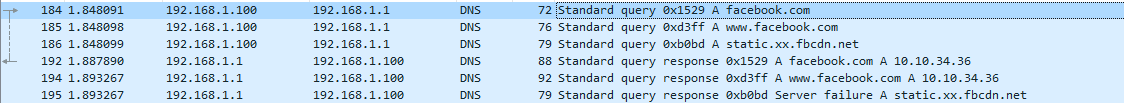
\includegraphics[width = 1.0 \textwidth]{images/1.png}
		\end{center}

سه درخواست اول از کامپیوتر من به روتر رفته‌اند و سه مورد بعدی جواب‌هایی هستند که از روتر به کامپیوتر من برگشته اند. مشاهده می‌کنیم آدرس آی‌پی که برای فیسبوک برگشته است
\lr{\Verb+10.10.34.36+}
است.

این آدرس آی‌پی جزو دسته آی‌پی‌های رزرو شده است که بین
\lr{\Verb+10.0.0.0+}
تا
\lr{\Verb+10.255.255.255+}
قرار دارد. این آدرس آی‌پی‌ها مربوط به شبکه‌های خصوصی هستند و عملا به سایت خاصی در اینترنت نگاشت نشده‌اند. این یعنی \lr{DNS} سرور، آدرسی را برای سایت \lr{Facebook} برگردانده که عملا مربوط به شبکه عمومی اینترنت نمی‌شود و یک آدرس در شبکه خصوصی است که عملا در کامپیوتر من وجود  نداشته و نتیجتا کروم با خطای
\lr {\Verb+This site can’t be reached+}
و
\lr{\Verb+ERR\_CONNECTION\_TIMED\_OUT+}
متوقف می‌شود.
	
	با بررسی تنظیمات مودم متوجه شدم که DNS-Server پیش‌فرض آن به صورت \lr{\Verb+46.224.1.220+} است که با \lr{IpLookup} کردن آن، متوجه می‌شویم که این آی‌پی متعلق به \lr{\Verb+ns5.hiweb.ir+} یعنی Nameserver «های‌وب» در ایران است و منطقی است که فیلترینگ روی این Nameserver داخلی اعمال شده باشد و در نتیجه DNS به آن نتیجه نامعتبری برای \lr{facebook.com} که یک سایت فیلتر شده است برگرداند.
	
	
	\item
	
	وضعیت درخواست DNS برای سایت اوراکل به صورت زیر است:
	
		\begin{center}
		
\includegraphics[width = 1.0 \textwidth]{images/2.png}
	\end{center}
	
	


وضعیت خروجی برگدانده شده برای آن به صورت زیر است:

\begin{latin}
	\begin{verbatim}
		Answers
		www.oracle.com: type CNAME, class IN, cname ds-www.oracle.com.edgekey.net
		Name: www.oracle.com
		Type: CNAME (Canonical NAME for an alias) (5)
		Class: IN (0x0001)
		Time to live: 497 (8 minutes, 17 seconds)
		Data length: 31
		CNAME: ds-www.oracle.com.edgekey.net
		ds-www.oracle.com.edgekey.net: type CNAME, class IN, cname e2581.dscx.akamaiedge.net
		Name: ds-www.oracle.com.edgekey.net
		Type: CNAME (Canonical NAME for an alias) (5)
		Class: IN (0x0001)
		Time to live: 451 (7 minutes, 31 seconds)
		Data length: 24
		CNAME: e2581.dscx.akamaiedge.net
		e2581.dscx.akamaiedge.net: type A, class IN, addr 23.14.117.40
		Name: e2581.dscx.akamaiedge.net
		Type: A (Host Address) (1)
		Class: IN (0x0001)
		Time to live: 497 (8 minutes, 17 seconds)
		Data length: 4
		Address: 23.14.117.40
		
	\end{verbatim}
\end{latin}
	
	جواب اول مشخص می‌کند که \lr{\Verb+www.oracle.com+} در اصل یک \lr{Alias} برای یک آدرس دیگر است.
	
	 جواب دوم مشخص می‌کند که آدرس مشخص شده بعدی یعنی
	 
	  \lr{\Verb+ds-www.oracle.com.edgekey.net+}
	  
	   هم یک \lr{Alias} برای آدرس دیگری است. آدرس نهایی یعنی \lr{\Verb+e2581.dscx.akamaiedge.net+} به یک آدرس آی‌پی واقعی مپ شده است. این آدرس ای‌پی یعنی \lr{\Verb+23.14.117.40+} مربوط به یکی از \lr{CDN} های شرکت \lr{Akamai} است. این \lr{CDN} در ترکیه واقع شده است و براساس موقعیت مکانی من که ایران بوده، نزدیک‌ترین \lr{CDN} تشخیص داده شده مربوط به کشور ترکیه بوده است. با این وجود در نهایت شاهد این هستیم که سایت \lr{Oracle} باز نمی‌شود و با خطاهای 
	\lr {\Verb+This site can’t be reached+}
	و
	\lr{\Verb+ERR\_CONNECTION\_TIMED\_OUT+}
	مواجه می‌شویم. این خطاها این بار به خاطر فیلترینگ نیستند بلکه به خاطر تحریم است.
	
	
		
	
	
	\item
	
	پیش از بررس نتایج باید بررسی کنیم که آی‌پی آدرس DNS-Server های شکن متعلق به کجاست. در سایت دو آی‌پی آدرس قرار گرفته است. اولین مورد \lr{\Verb+178.22.122.100+} است که متعلق به شرکت آسیاتک (\lr{Asiatech Data Transmission company}) بوده و دومین آی‌پی \lr{\Verb+185.51.200.2+} است که متعلق به شرکت مهندسی صفرویک پرداز (\lr{Sefroyek Pardaz Engineering Co. LTD}) است.
	
	
	
\end{enumerate}
\end{document}



